%=============================================================================
% Thesis Template in LaTex
%
% File:  Kostenstruktur -- Fallstudie
% Author(s): Jürgen Hackl <hackl@ibi.baug.ethz.ch>
%            Clemens Kielhauser <kielhauser@ibi.baug.ethz.ch>
%
% Creation:  27 Jan 2014
% Time-stamp: <Tue 2013-08-13 20:14 juergen>
%
% Copyright (c) 2014 Infrastructure Management Group (IMG)
%               http://ibi.ethz.ch
%
% More information on LaTeX: http://www.latex-project.org/
%=============================================================================

% Unterkapitel Kostenstruktur
% ---------


\subsection*{Unterhaltskosten}
\label{sub:Unterhalt}

Die Berechnung der Unterhaltskosten $K_{U}$ der Infrastruktur erfolgt gemäss der Formel \ref{eq.2}. Sie setzen sich zusammen aus den einmaligen Investitionskosten für den Bau der Infrastruktur $K_{Bau}$ und den jährlich anfallenden Wartungskosten $K_{Wartung,t}$.

\begin{equation}
K_{U} = K_{Bau} + \sum_{t=0}^T \  K_{Wartung,t}  \label{eq.2} \\ 
\end{equation}

\begin{align*}
	  k &=
      \begin{cases}
        \begin{aligned}
          & 1 \\
          & 2
        \end{aligned} &
        \begin{aligned}
         & \text{für}\ \thinspace \\
         & \text{für}\ \thinspace
        \end{aligned}
        \begin{aligned}
          & Strasse \\
          & Unterführung
        \end{aligned}
      \end{cases} \\
\end{align*}

{\setstretch{0.6}
wobei:
\begin{conditions}
 K_{U}      	     			&  Totale Unterhaltskosten für $T$ Jahre  \\
 K_{Bau}           			    &  Baukosten der Variante     \\
 K_{Wartung,t}                  &  Wartungskosten pro Jahr     
\end{conditions}
}

Die Berechnung der Wartungskosten erfolgt ahand Formel \ref{eq.3}. Die Einheitskosten für den Bau und die Wartung werden nachfolgend erläutert.

\begin{equation}
K_{Wartung,t} = \sum_{t=1}^2 \ EK_{Wartung,k} \cdot s_{k} \cdot b_{k}  \label{eq.3} 
\end{equation}

{\setstretch{0.6}
wobei:
\begin{conditions}
 EK_{Wartung,k}      	     	&  Einheitskosten pro $m^2$   \\
 s_k	    	     			&  Länge der Infrastruktur in $m$ \\
 b_k	    	     			&  Breite der Infrastruktur in $m$   \\
 k								&  Art der Infrastruktur  
\end{conditions}
}

\newpage

\begin{IMleftrightskip}
Die Erstellung zweier neuer Radstreifen à je 1.5 $m$ Breite kostet pro Laufmeter 850 CHF. Die Investitionskosten pro Quadratmeter für den Bau einer Velounterführung unter dem Lastfall Eisenbahn, betragen 3750 CHF. Der Bau der Zufahrtsrampen zu den Velounterführungen kostet pro Rampe 130'000 $CHF$. (\cite{Baukosten2010})
Die Wartungskosten habe ich nach einem Gespräch mit Herr Dr. Martani wie folgt angesetzt. Für die Instandhaltung der Strasse, inklusive der Fahrradstreifen und der Fussgängerwege fallen jährlich 5 \thinspace $\frac{CHF}{m^2}$ an. Die wartungsintesivere Infrastruktur der Unterführung wird jährlich mit 30 \thinspace $\frac{CHF}{m^2}$ instand gehalten. \\
\end{IMleftrightskip}

Diese Kosten sind hauptsächtlich von der Auslastung der Infrastruktur und vom Gewicht der Fahrzeuge, die sie befahren, abhängig. Da diese Kosten im Vergleich zu den anderen Kostenpositionen deutlich geringen ausfallen, verzichte ich auf eine Variation dieser Parameter über den betrachteten Zeithorizont. Die nachfolgende Tabelle \ref{tab:t-04-03-01-Unterhalt} fasst die für die Besitzer anfallenden Einheitskosten zusammen.

%=============================================================================
% Thesis Template in LaTex
%
% File:  t-05-01-IsingModel.tex -- Table for the Ising
% Author(s): Juergen Hackl <hackl@ibi.baug.ethz.ch>
%            Clemens Kielhauser <kielhauser@ibi.baug.ethz.ch>
%
% Creation:  27 Jan 2014
% Time-stamp: <Tue 2013-08-13 20:14 juergen>
%
% Copyright (c) 2014 Infrastructure Management Group (IMG)
%               http://ibi.ethz.ch
%
% More information on LaTeX: http://www.latex-project.org/
%=============================================================================

\begin{table}[h!]
\flushleft
%\center
\renewcommand{\arraystretch}{1.4}
%\captionsetup{justification=centering}

\begin{tabular}{ @{} lc|ccc @{} }
                 &                         & Fahrbahn  & Veloweg  & Unterführung \\ \hline
Unterhaltskosten &$\frac{CHF}{m^2 \ Jahr}$ &     5     &     5    &      30        \\
Baukosten        &$\frac{CHF}{m}$ 		   &     -     &   850    &     18'900        
\end{tabular}
\caption{Bau- und Unterhaltskosten}
\label{tab:t-04-03-01-Unterhalt}
\end{table}

%\begin{table}[h!]
%\flushleft
%\renewcommand{\arraystretch}{1.4}
%\small\renewcommand{\arraystretch}{1.2} 
%
%
%\begin{tabular}{@{}p{3.3cm} p{4cm} p{1cm} r l @{}} \\   
%\toprule
%\textbf{Interessensgruppe} & \textbf{Kostentyp} & \textbf{Symbol} & \multicolumn{2}{c}{\textbf{Einheitskosten}} 			\\
%\midrule

%\bottomrule

%\end{tabular}

%\end{table}


%=============================================================================
% EOF
%

%%% Local Variables:
%%% mode: latex
%%% TeX-master: "../guidelines"
%%% End:



\newpage

\subsection*{Betriebskosten}
\label{sub:Betrieb}


Die Betriebskosten $K_{B}$ die für die Nutzer der Infrastruktur, für den betrachteten Zeitraum von $T$ Jahren, anfallen, werden gemäss Formel \ref{eq.6} berechnet. So werden die Betriebskosten aus der Multiplikation der Anzahl Nutzer und der zurückgelegten Distanz mit den Einheitskosten pro Fahrzeugkilometer ermittelt.
Diese sogenannten Fahrzeugsbetriebkosten sind im Rahmen dieser Optimierung, als die jährlich pro Nutzer anfallenden Wartungskosten definiert und sind somit die Kosten, die für die Instandsetzung und den Betrieb eines Fahrzeugs, bei benützung der Infrastruktur, entstehen können. Diese setzen sich zusammen aus den Kosten der Arbeitssstunden für die Instandsetzung sowie der Kosten für die Ersatz- und Verschleissteile.
 
Diese Kosten sind abhängig von der Qualität des Fahrbahnbelags, von der Ausführung der Infrastruktur und von der Kapazität der Infrastruktur. Weiter ist ein entscheidender Faktor in der Bestimmung der Fahrzeugbetriebskosten die Strassengeometry. Diese beinhaltet die Anzahl und Form der Kurven, die Steigungen sowie die Breite der Strasse und die daraus resultierende Möglichkeit des sicheren Überholens. Die Anzahl an Kreuzungsstellen und die davon abhänginge Anzahl an Brems- und Beschleunigungsmanöver haben einen direkten Einfluss auf den Verschleiss der Mechanik des Fahrzeugs. So werden im Falle des Fahrrads die Kette und die Bremsbeläge durch vermehrtes Bremsen und Anfahren verstärkt abgenutzt und im Falle des Autos erhöhen sich die Betriebskosten bei vermehrtem \textit{Stop-and-Go} Verkehr.

\begin{equation}
K_{B} =  \sum_{t=0}^T \Biggl[ \sum_{j=1}^2 \ EK_{B,j} \cdot s_{k} \cdot DTV_{j} \Biggr]  \label{eq.6} \\
\end{equation}

{\setstretch{0.6}
wobei:
\begin{conditions}
 K_{B}			   &  Totale Fahrzeugbetriebskosten \\
 EK_{B,j}	       &  Einheitskosten pro $km$ \\
 s_j	    	   &  Länge der Infrastruktur nach Fahrzeugtyp in $km$ 
\end{conditions}
}

Die Einheitskosten des Fahrzeugsbetrieb sind mehrheitlich abhängig von der Entwicklung der Fahrzeugtechnologie und der Verarbeitungsqualität. 
Die Einführung autonomer Fahrzeuge, würde diese Kostenposition in Zukunft obsolet machen. Jedoch ist die Zulassung solcher Fahrzeuge für den innerstädtischen Verkehr nicht vor 2050 zu erwarten. Da dies, erst am Ende meines betrachteten Zeithorizont eine Rolle spielen wird und der Effekt der die einführung von autonomen Fahrzeugen auf die Betriebskosten des Nutzers nicht eindeutig beziffert werden kann, verzichte ich auf eine Variation dieser Parameter. Somit bleiben die Einheitskosten des Fahrzeugbetriebs über den betrachteten Zeithorizont konstant.
Zur Vereinfachung der Berechnung, werden die entstehenden Betriebskosten anhand der nachfolgenden Referenzwerte ermittelt.
Die Kosten der Arbeitsstunden sowie die Kosten der Materialien werden zusammengefasst als die Einheitskosten $EK_{B}$ für den Fahrzeugbetrieb.
Diese betragen pro Auto 0.7 $CHF$ pro $km$ und pro Velo 0.15 $CHF$ pro $km$ (Quelle: TCS und eigene Erfahrungswerte). 



\subsection*{Reisezeitkosten}
\label{sub:Reisezeit}

Erleidet man beim befahren einer Infrastruktur einen Zeitverlust, entsteht dem Nutzer einen Schaden. Zieht man in betracht, dass der Nutzer in dieser Zeit hätte arbeiten können oder Freizeit verbringen, kann dieser Schaden monäter beziffert werden. Beispiele hierfür wären, die Mehrkosten eines Spediteurs aufgrund des Zeitverlust oder die Mehrkosten auf einem Ausflug, durch eine verpasste Verbindung .
Diese Kosten werden indirekt vom Zustand des Fahrbahnbelags beeinflusst. Vom Zustand des Fahrbahnbelags ist die Reisegeschwindigkeit und somit die Zeit die benötigt wird, eine gewisse Strecke zurückzulegen, abhängig.

Die Berechnung der totalen Reisezeitkosten $K_{TT}$ erfolgt gemäss Formel \ref{eq.4} in Anlehnung an die Berechnung der \textit{Travel time cost} aus \cite[S.643]{Adey2012}.

\begin{equation}
K_{TT} = \sum_{t=0}^T \Biggl[ \sum_{j=1}^2 \ DTV_{j} \cdot t_{j} \cdot EK_{TT,j} \Biggr]  \label{eq.4}
\end{equation}

\begin{align*}
	 j &=
      \begin{cases}
        \begin{aligned}
          & 1 \\
          & 2
        \end{aligned} &
        \begin{aligned}
         & \text{für}\ \thinspace \\
         & \text{für}\ \thinspace
        \end{aligned}
        \begin{aligned}
          & MIV \\
          & Velo
        \end{aligned}
      \end{cases} \\
\end{align*}

{\setstretch{0.6}
wobei:
\begin{conditions}
 K_{TT}		 	 &  Totale Reisezeitkosten für $T$ Jahre  \\
 DTV_{j}    	 &  Tägliches Verkehrsaufkommen nach Fahrzeugtyp \\
 t_{j} 			 &  Zeitverlust nach Fahrzeugtyp \\
 EK_{TT,j} 		 &  Einheitskosten der verlorenen Zeit in $CHF/h$ \\
 j				 &  Art des Fahrzeugs   
\end{conditions}
}

\begin{IMleftrightskip}
Die Zeit die man benötigt eine bestimmte Strecke zurück zu legen ist abhängig von der gefahrenen Geschwindigkeit $v_{j}$, welche wiederum durch Zustand der Strasse sowie von der Kapazität $C_{j}$ der Infrastruktur, bestimmt wird. Diese Approximation ermöglicht es mir, die verlorene Zeit, gemäss \ref{eg.5} zu berechnen, wobei die Parameter $\alpha$ und $\beta$ die Strasseneigenschaften repräsentieren.  
\end{IMleftrightskip}

\newpage

\begin{equation}
t = \frac{s_{k}}{v_{j}} \Biggl( 1 + \alpha \Bigl(\frac{DTV_{j}}{C_{j}} \Bigr)^\beta \Biggr) \label{eg.5} 
\end{equation}

{\setstretch{0.6}
wobei:
\begin{conditions}
 v_{j}			 &  Gefahrene Geschwindigkeit nach Fahrzeugtyp \\
 \alpha			 &  (0.15 vorgeschlagen nach (\cite{Adey2012}))  \\
 \beta			 &  (4 vorgeschlagen nach (\cite{Adey2012}))  \\
 C_{j}			 &  Kapazität der Infrastruktur pro Tag nach Fahrzeugtyp  \\
 j				 &  Art des Fahrzeugs   
\end{conditions}
}

\begin{IMleftrightskip}
Der Bahnübergang Brunnenstrasse ist augfrund des regen S-Bahn Verkehrs und somit dichten Fahrplans am Bahnhof Uster, pro Stunde bis zu 40' geschlossen. Daraus resultiert gemäss STEK pro Benutzer des Bahnübergangs eine durchschnittliche Wartezeit von 5 Minuten, was einem einem Zeitverlust von 0.0833 $h$/Fahrzeug entspricht. Um die durchschnittliche Wartezeit in die Berechnung der Reisezeitkosten miteinzubeziehen, wird der berechnete Zeitverlust $t_{j}$ um diesen Faktor vergrössert. \\
Der effektive beim benutzen des Bahnübergangs anfallende Zeitverlust nach Formel \ref{eg.5} ist somit hauptsächlich von der Schliesszeit der Bahnschranken abhängig. Die durchschnittliche Wartezeit pro Nutzer setzt sich aus der Zeit die ein Zug für die Durchfahrt benötigt und einem Faktor der die Zeit für die Öffnung der Schranken sowie die Wartzeit aufgrund eines allfällige enstehehden Rückstaus repräsentiert, zusammen. Die durchschnittliche Durchfahrtszeit eines Zuges beträgt gemäss (\cite{STEK}) 3' und der vorgängig erläuterte Faktor wird für die Berechnung, nach konsultation verschiedener Literaturen, mit 2' angesetzt. 
Der Einfluss der Veränderung des Fahrplans wird im Abschnitt \ref{subsec:Sensitivitätsanalyse} weitere untersucht. 
\end{IMleftrightskip}

Die Einheitskosten des Zeitverlustes $EK_{TT,j}$ pro Velofahrer betragen 19.70 $CHF/h$. Um denn durchschnittlichen Auslastungsgrad von 1.6 Personen pro Auto  zuberücksichtigen, wird dieser Wert mit dem Faktor 1.6 multipliziert. Somit betragen die Einheitskosten des Zeitverlustes für den motorisierten Individualverkehr 31.52 $CHF/h$ pro Auto. (\cite{Adey2012}) (\cite{Mikrozensus2015})


Die nachfolgenden Tabelle \ref{tab:t-04-03-02-Nutzerkosten} fast die für die Nutzer anfallenden Einheitskosten zusammen.
%=============================================================================
% Thesis Template in LaTex
%
% File:  t-05-01-IsingModel.tex -- Table for the Ising
% Author(s): Juergen Hackl <hackl@ibi.baug.ethz.ch>
%            Clemens Kielhauser <kielhauser@ibi.baug.ethz.ch>
%
% Creation:  27 Jan 2014
% Time-stamp: <Tue 2013-08-13 20:14 juergen>
%
% Copyright (c) 2014 Infrastructure Management Group (IMG)
%               http://ibi.ethz.ch
%
% More information on LaTeX: http://www.latex-project.org/
%=============================================================================

\begin{table}[h!]
\center
\renewcommand{\arraystretch}{1.4}
\begin{tabular}{l|c|c}
            & Reisezeitkosten   $\frac{CHF}{h}$	& Betriebskosten   $\frac{CHF}{Pkm}$         \\ \hline
Velo	    &       19.70          			    &      0.15       			                \\
MIV         &      	31.52          		        &      0.7                    
\end{tabular}
\caption{Übersich der Nutzerkosten}
\label{tab:t-04-03-02-Nutzerkosten}
\end{table}

%\begin{table}[h!]
%\flushleft
%\renewcommand{\arraystretch}{1.4}
%\small\renewcommand{\arraystretch}{1.2} 
%
%
%\begin{tabular}{@{}p{3.3cm} p{4cm} p{1cm} r l @{}} \\   
%\toprule
%\textbf{Interessensgruppe} & \textbf{Kostentyp} & \textbf{Symbol} & \multicolumn{2}{c}{\textbf{Einheitskosten}} 			\\
%\midrule

%\bottomrule

%\end{tabular}

%\end{table}


%=============================================================================
% EOF
%

%%% Local Variables:
%%% mode: latex
%%% TeX-master: "../guidelines"
%%% End:



\newpage


\subsection*{Umwelkosten}
\label{subsec:Environment}


Die gemäss Formel \ref{eq.7} berechneten Kosten der Belastung der Umwelt $K_{E}$ (\textit{Englisch}: Environment), bestehen aus den Kosten durch die Schadstoffbelastung$K_{S}$ und der Kosten durch die Lärmbelastung $K_{L}$. Sie repräsentieren die Schäden, die von der Allgemeinheit getragen werden, durch den motorisierten Individualverkehr an der Umwelt und  

\begin{equation}
K_{E} = \sum_{t=0}^T \ \biggl(K_{L,t} + K_{S,t} \biggr)  \label{eq.7} \\
\end{equation}

{\setstretch{0.6}
wobei:
\begin{conditions}
 K_{E}		   &  Totale Umwelkosten  \\
 K_{L,t}       &  Kosten durch die Lärmbelastung pro Jahr  \\
 K_{S,t}       &  Kosten durch die Schadstoffbelastung pro Jahr 
\end{conditions} 
}

Die \textbf{Lärmbelastung} durch den Verkehr verursacht Kosten $K_{L}$, die von der Allgemeinheit getragen werden. Die nach Formel \ref{eq.9} berechneten Kosten setzen sich einerseits aus den Mietzinsausfälle, da eine erhöhte Lärmbelastung zu einer Reduktion des Mietzins führt und andererseits aus den durch den Lärm verursachten Gesundheitskosten, zusammen. 
Diese Gesundheitskosten entstehen durch die Störung und Beeinträchtigung der Anwohner in Form von Kopfschmerzen, Bluthochdruck, Schlafstörrungen sowie psychischer Belastung. (\cite{Ecoplan2007}) \\

\begin{equation}
K_{L,t} = EK_{L} \cdot DTV_{MIV,t} \cdot s_{i}  \label{eq.9} \\
\end{equation}

{\setstretch{0.6}
wobei:
\begin{conditions}
 EK_{L}         	&  Einheitskosten der Lärmbelastung pro Fahrzeugkilometer \\
 DTV_{MIV,t}    	&  Durchschnittliche tägliche Verkehrsaufkommen im Jahr $t$  \\
 s_{MIV}          	&  Zurückgelegte Distanz in $[km]$ pro Fahrzeug 
\end{conditions} 
}

\begin{IMleftrightskip}
Der Lärm entsteht mehrheitlich durch Motorengeräusche sowie der Abrollgeräusche der Reifen. Eine Schweirigkeit bei der bezifferung des Ausmasses dieser Kosten, ist die oben erwähnten Auswirkungen des Lärms auf die Allgemeinheit zu quantifizieren. (\cite{Adey2012})
Das Ausmass des entstandenen Schadens, ist somit vollständig von der Fahrzeugtechnologie abghängig. Eine Reduktion der Lärmbelastung durch Veränderung der Reifentechnologie, ist im betrachten Zeithorizont nicht zuerwarten. Die Einheitskosten der Lärmbelastung $EK_{L}$ werden infolge, anhand des Berichts zu den externen Lärmkosten des Strassenverkehrs, mit 0.0149 $CHF$/Fahrzeugkilometer angenähert. (\cite{Lärm2000})
\end{IMleftrightskip}



Die in Formel \ref{eq.8} dargestellten Kosten der \textbf{Schadstoffbelastung} $K_{S}$, sind die Kosten die der Allgemeinheit durch die Emissionen von Motorfahrzeugen entstehen. Diese Schäden können neben gesundheitlichen Problemen für die Anwohner und Nutzer der Strasse und der Beeinträchtigung des Pflanzenwachstums entlang der Infrastruktur auch die Reduktion des Werts einer Liegenschafts sein. 

\begin{equation}
K_{S,t} = EK_{S} \cdot DTV_{MIV,t} \cdot s_{i} \biggl( 1 - \Phi_{E-Auto,t} \biggr)   \label{eq.8} \\
\end{equation}

{\setstretch{0.6}
wobei:
\begin{conditions}
 EK_{S}         	&  Einheitskosten der Schadstoffbelastug pro Fahrzeugkilometer \\
 DTV_{MIV,t}    	&  Durchschnittliche tägliche Verkehrsaufkommen des MIV im Jahr $t$  \\
 s_{MIV}          	&  Zurückgelegte Distanz in $[km]$ \\
 \Phi_{E-Auto,t}    &  Marktanteil E-Autos am $DTV_{MIV,t}$ im Jahr $t$ 
\end{conditions} 
}

\begin{IMleftrightskip}
Die entstehenden Kosten der Schadstoffbelastung werden mehrheitlich durh die gefahrenen Geschwindigkeit und den Verkehrsfluss beeinflusst. So nimmt die Belastung der Luft durch Schadstoffe deutlich zu, wenn vermehrt im \textit{Stopp and Go-Verkehr} gefahren wird. Da für das modellieren dieser Beziehung im Rahmen meiner Untersuchungen nicht genügend Zeit zur Verfügung stand, bestimme ich die Kosten der Schadstoffbelastung  anhand des Schlussberichts zu den externen Kosten im Strassenverkehr (\cite{Ecoplan2007}). Somit betragen die, für die Öffentlichkeit anfallenden Einheitskosten $EK_{S}$ 0.0345 CHF/Fahrzeugkilometer.\\
Da elektronisch angetrieben Fahrzeuge keine Emissionen verursachen und demzufolge keine Kosten infolge Schadstoffbelastung, wird der Anteil an E-Autos \( \Phi_{E-Auto,t} \) beim berechnen der Umweltkosten vom täglichen Verkehrsaufkommen abgezogen.  
\end{IMleftrightskip}

%=============================================================================
% Thesis Template in LaTex
%
% File:  t-05-01-IsingModel.tex -- Table for the Ising
% Author(s): Juergen Hackl <hackl@ibi.baug.ethz.ch>
%            Clemens Kielhauser <kielhauser@ibi.baug.ethz.ch>
%
% Creation:  27 Jan 2014
% Time-stamp: <Tue 2013-08-13 20:14 juergen>
%
% Copyright (c) 2014 Infrastructure Management Group (IMG)
%               http://ibi.ethz.ch
%
% More information on LaTeX: http://www.latex-project.org/
%=============================================================================

\begin{table}[h!]
\center
\renewcommand{\arraystretch}{1.4}
\begin{tabular}{l|c}
            			& Umweltkosten   $\frac{CHF}{Pkm}$	       \\ \hline
Schadstoffbelastung	    &       0.0345          		                \\
Lärmbelastung           &      	0.0149          		                       
\end{tabular}
\caption{Übersich der Nutzerkosten}
\label{tab:t-04-03-01-Umwelt}
\end{table}

%\begin{table}[h!]
%\flushleft
%\renewcommand{\arraystretch}{1.4}
%\small\renewcommand{\arraystretch}{1.2} 
%
%
%\begin{tabular}{@{}p{3.3cm} p{4cm} p{1cm} r l @{}} \\   
%\toprule
%\textbf{Interessensgruppe} & \textbf{Kostentyp} & \textbf{Symbol} & \multicolumn{2}{c}{\textbf{Einheitskosten}} 			\\
%\midrule

%\bottomrule

%\end{tabular}

%\end{table}


%=============================================================================
% EOF
%

%%% Local Variables:
%%% mode: latex
%%% TeX-master: "../guidelines"
%%% End:


\newpage

\subsubsection*{Marktanteil E-Autos}
\label{subsubsec:Marktanteil}

Im Jahr 2019 betrug der Marktanteil der E-Autos am Personenwagenbestand in der Schweiz 0.621 \%. Für das Jahr 2050 prognostiziere ich, nach konsultation verschiedenster Literaturen, dass der Marktanteil der E-Autos in der SChweiz bei 90 \% zu liegen kommt. (\cite{Bestand2019}) \\
Um die Berechnung zu vereinfachen nehme ich an, dass das Wachstum linear erfolgt. Somit beträgt der jährliche Anstieg des Marktanteils der E-Autos am Personenwagebestand 2.88 \%. Die Resultate meiner Berechnungen des jährlichen Marktanteils der E-Autos am Strassenfahrzeugbestand \( \Phi_{E-Auto} \) ist in der nachfolgenden Abbildung \ref{img:Marktanteil} festgehalten. 

\begin{figure}[h!]
	\centering
	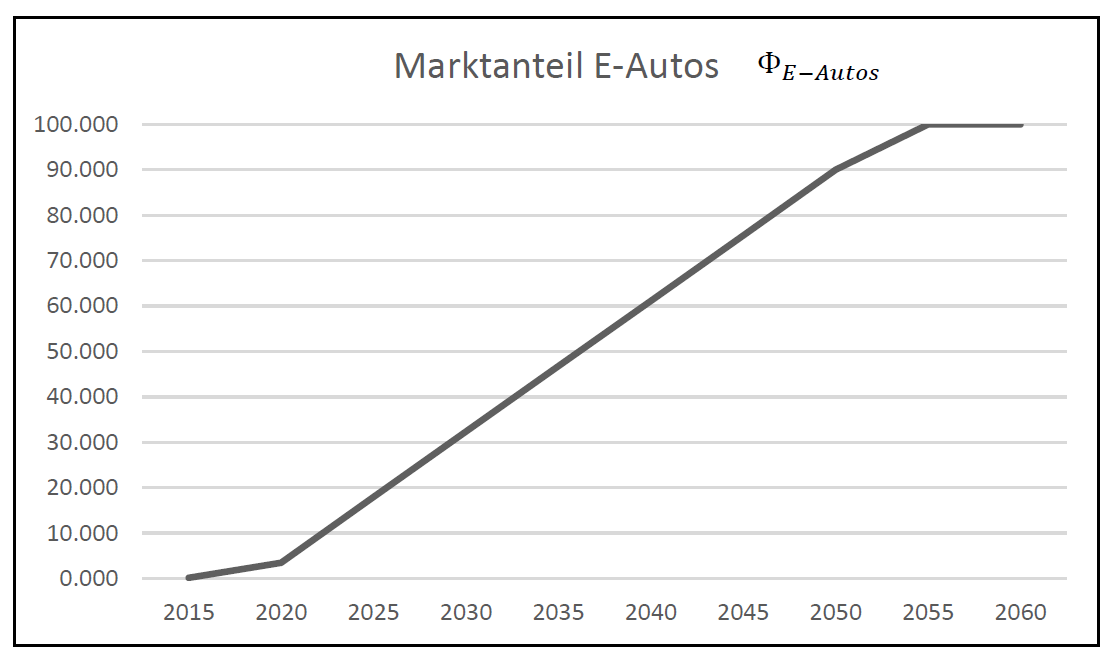
\includegraphics[width=.6\textwidth]{figures/04-04-01-MarktanteilE-Auto}
	\caption[Marktanteil E-Autos]{Marktanteils der E-Autos am Strassenfahrzeugbestand}
	\label{img:Marktanteil}
\end{figure}



\pagebreak


\subsection*{Unfallkosten}
\label{subsec:Unfall}

Die totalen Unfallkosten $K_{A}$ welche von der Allgemeinheit für den betrachteten Zeitraum getragen werden müssen, werden gemäss Formel \ref{eq.10} berechnet. So ergibt sich aus der Multiplikation der Anzahl Fahrzeuge und der Unfallwahrscheinlichkeit, die Anzahl Unfälle auf der Infrastruktur. Die Anzahl Unfälle multipliziert man, um die gesamten Unfallkosten zu ermittelt, mit den Einheitskosten der jeweiligen Unfalltypen.

In Betracht gezogen werden drei verschiedene Unfaltypen [$a$,$b$,$c$].
Unfälle mit entstandenen Sachschäden und leichtverletzten Personen werden in die Kategorie $a$ eingeteilt. Für Unfälle mit schwerverletzten Beteiligten wird die Kategorie $b$ definiert und für Unfälle mit Todesfolge die Kategorie $c$. 
Die Kategorien unterscheidenen sich in der Häufigkeit des Unfalls pro Fahrzeug \( \gamma_{j,n} \), sowie der entstehenden Einheitskosten pro Unfall $EK_{j,n}$.

\begin{IMleftrightskip}
Wichtig anzumerken ist, dass die ermittelten Unfallrisiken die Anzahl Unfälle eines Unfalltyps pro Personenkilometer darstellen. Das bedeuted, dass für die Berechnung der Personenkilometer der mototrisierten Fahrzeuge, der Auslastungsgrad gemäss (\cite{Mikrozensus2015}) in Betracht gezogen werden muss. Somit wird in der Berechnung der Unfallkosten der $DTV_{MIV}$ mit einem Faktor 1.6 multipliziert.
\end{IMleftrightskip}

\begin{equation}
K_{A} = \sum_{t=0}^T \Biggl[ \sum_{j=1}^2 \Bigl( \sum_{n=a}^c \ EK_{j,n} \cdot \gamma_{j,n} \Bigr) \cdot DTV_{j} \cdot s_j \Biggr] 
\label{eq.10}
\end{equation}

\begin{align*}
      n &=
      \begin{cases}
        \begin{aligned}
          & a  \\
          & b \\
          & c
        \end{aligned} &
        \begin{aligned}
         & \text{für}\ \thinspace \\
         & \text{für}\ \thinspace \\
         & \text{für}\ \thinspace
        \end{aligned}
        \begin{aligned}
          & {Sachsch"aden\,und\,Leichtverletzte} \\
          & {Schwerverletzte} \\
          & {Todesfall}
        \end{aligned}
      \end{cases}  \\
      j &=
      \begin{cases}
        \begin{aligned}
          & 1 \\
          & 2
        \end{aligned} &
        \begin{aligned}
         & \text{für}\ \thinspace \\
         & \text{für}\ \thinspace
        \end{aligned}
        \begin{aligned}
          & Velo \\
          & Auto
        \end{aligned}
      \end{cases} \\
\end{align*}

{\setstretch{0.6}
wobei:
\begin{conditions}
 K_{A}	 		 &  Totale Unfallkosten \\
 EK_{j,n} 		 &  Einheitskosten pro Unfall nach Fahrzeugtyp \\
 \gamma_{j,n} 	 &  Unfallwahrscheinlichkeit nach Fahrzeugtyp \\
 DTV_{j}		 &  Tägliches Verkehrsaufkommen nach Fahrzeugtyp \\
 s_j	    	 &  Länge der Infrastruktur nach Fahrzeugtyp in $km$  \\
 n 				 &  Unfallart  \\
 j          	 &  Art des Fahrzeugs  
\end{conditions}
} 

Die Gefahrenlage auf der Infrastruktur wird von mir, durch die Berechnung der Unfallrisiken anhand der gesamtschweizerischen Unfalldaten, abgeschätzt.
Die effektive Gefahrensituation wird, dadurch jedoch nicht berücksichtig. Um diese berücksichtigen zu können, müssten die Unfalldaten der Brunnenstrasse verwendet werden. Diese sind jedoch unvollständig und daher verwende ich zur Berechnung der Unfallrisken die Unfalldaten für die ganze Schweiz. 
Da die Entwicklung der Verkehrssicherheit von verschiedensten Faktoren abhängig ist, habe ich mich im Rahmen dieser Untersuchungen aus Zeitgründen dazu entschieden, die Entwicklung der Unfallrisiken über den betrachteten Zeithorizont nicht zu variieren. 
Eine Untersuchung des Effekts der Veränderung der Unfallrisiken in Abhängigkeit der gebauten Variante erfolgt im Abschnitt \ref{subsec:Sensitivitätsanalyse}.

\newpage

\subsubsection*{Unfallrisiko}
\label{subsubsec:Unfallrisiko}


Das Risiko im Strassenverkehr einen Unfall zu erleiden, ist von verschiedenen Faktoren abhängig. Ich berechne das sogenannten Unfallrisiko, also die Wahrscheinlichkeit im Strassenverkehr einen Unfall zu erleiden, mit den Angaben zu den Leistungen des privaten Personenverkehrs auf der Strasse und der Strasenverkehrsunfall-Statistik. So teile ich die Anzahl Unfälle nach Unfallart, durch die Verkehrsleistungen der verschiedenen Verkehrsteilnehmer und erhalte so das Risiko eines Unfalls pro Personenkilometer.  Diese Unfallwahrscheinlichkeit bezeichne ich mit  \( \gamma_{j,n} \).

Das Unfallrisiko des MIV ermittle ich aus den Unfallzahlen und den Verkehrsleistung der Personenwagen und der Motorräder in der Schweiz. Die Gesamtleistung der Personenwagen in der Schweiz, lag im Jahr 2018 bei 96.9 Mrd. Personenkilometer. Die Verkehrsleistung der Motorräder, inklusive Motorfahrräder und schnelle E-Bikes lag hingegen bei 2.2 Mrd. Personenkilometer. So ergibt sich für die den MIV eine Verkehrsleistung von 99.1 Mrd. Personenkilometer für das Jahr 2018. (\cite{Verkehrsleistung2019})\\
Die Unfallzahlen des MIV setzten sich aus den Unfallzahlen der Personenwagen, der Motorräder inklusive Motorfahrräder und schnelle E-Bikes zusammen. Im Jahr 2018 erlagen ingsesamt 116 Personen den Folgen eines Unfalls mit Beteiligung des MIV, 1898 Personen wurden schwer- und 12'106 Personen leicht verletzt. (\cite{Unfall2019})\\
Aus diesen Angaben habe ich die in Tabelle \ref{tab:t-06-01-Unfallrisiko} aufgelisteten Unfallrisiken ermittelt, indem ich die Anzahl Unfälle durch die Verkehrsleistungen geteilt habe.

Für den Langsamverkehr, den ich unter dem Begriff \textit{Velo} zusammenfasse, ergibt sich das selbe Vorgehen bei der Berechung der Unfallrisiken. So lag die Verkehrsleitung im Jahr 2018, der Velofahrer und langsamen E-Bikes, bei 2'520 Mio. Personenkilometer. (\cite{Verkehrsleistung2019}) \\
Im Jahr 2018 verunfallten in Zusammenhang mit dem Langsamverkehr, sprich mit den Velos oder den langsamen E-Bikes, 26 Personen tödlich. Im selben Zeitraum wurden 878 Personen schwer- und 2815 Personen leicht verletzt. (\cite{Unfall2019})
Wie für das Unfallrisiko des MIV habe ich aus diesen Angaben die Unfallrisiken der verschiedenen Unfalltypen für die Verkehrsteilnehmer des Langsamverkehrs ermittelt. Die berechneten Risiken sind in Tabelle \ref{tab:t-06-01-Unfallrisiko} für die verschiedenen Fahrzeuge $j$ und Unfalltypen $n$ zusammengefasst.

%=============================================================================
% Thesis Template in LaTex
%
% File:  t-05-01-IsingModel.tex -- Table for the Ising
% Author(s): Juergen Hackl <hackl@ibi.baug.ethz.ch>
%            Clemens Kielhauser <kielhauser@ibi.baug.ethz.ch>
%
% Creation:  27 Jan 2014
% Time-stamp: <Tue 2013-08-13 20:14 juergen>
%
% Copyright (c) 2014 Infrastructure Management Group (IMG)
%               http://ibi.ethz.ch
%
% More information on LaTeX: http://www.latex-project.org/
%=============================================================================

\begin{table}[hbt!]
\center
%\small\renewcommand{\arraystretch}{1.2} 
%
%
\begin{tabular}{@{}p{2.6cm} p{3.3cm} p{3.3cm} p{3.3cm}@{}} \\   
\toprule
\textbf{Fahrezugtyp\textsubscript{k}} & \textbf{Unfalltyp\,a} & \textbf{Unfalltyp\,b} & \textbf{Unfalltyp\,c} \\
\midrule
MIV      & \(1.317\,\mathrm{10^{-6}}\) $\frac{Unf"alle}{Pkm}$ & \(9.116\,\mathrm{10^{-8}}\) $\frac{Unf"alle}{Pkm}$ & \(4.7243\,\mathrm{10^{-9}}\) $\frac{Unf"alle}{Pkm}$ \\
Velo	 & \(3.818\,\mathrm{10^{-6}}\)  $\frac{Unf"alle}{Pkm}$ & \(2.643\,\mathrm{10^{-7}}\)  $\frac{Unf"alle}{Pkm}$ & \(1.37\,\mathrm{10^{-8}}\)  $\frac{Unf"alle}{Pkm}$  \\

\bottomrule

\end{tabular}
\caption[Tabelle der Unfallrisiken]{Tabelle der Unfallrisiken $\gamma_{k,n}\,\Bigl[\frac{Unf"alle_{k,n}}{Pkm_{k}}\Bigl]$}
\label{tab:t-06-01-Unfallrisiko}
\end{table}


%=============================================================================
% EOF
%

%%% Local Variables:
%%% mode: latex
%%% TeX-master: "../guidelines"
%%% End:




Nach der ausführlichen Betrachtung verschiedenster Literaturen zum Thema: \textit{Kosten die durch Strassenverkehrsunfälle entstehen} und einem Gespräch mit Herr Dr. Martani, habe ich für die Berechnung der Unfallkosten im Rahmen dieser Untersuchung, die folgenden Einheitskosten der verschiedenen Unfalltypen festgelegt.

\paragraph{Katergorie $a$} Die Einheitskosten pro Unfall der Kategorie $a$ setzen sich aus den entstandenen Sachschäden und den Arbeits- und Materialkosten der Reperatur eines Fahrzeugs zusammen. Das durchschnittliche Alter eines Personenenwagens in der Schweiz liegt bei 8.5 Jahren und der durschnittliche Wert eines solchen Fahrzeuge liegt gemäss TCS bei 15'000 CHF. Die Kosten der Behandlung der leichtverletzter Personen wird in dieser Betrachtung, aufgrund ihrer geringen grösse vernachlässigt, weshalb die pro Unfall enstehenden Kosten der Kategorie $a$ mit 15'000 CHF/Unfall angesetzt, werden.

\paragraph{Kategorie $b$} Die Kosten die aufgrund eines Unfalls der Kategorie $b$ entstehen, werden durch die anfallenden Behandlungskosten der verunfallten Person dominiert. Die Kosten durch den Erwerbsausfall für die Dauer der Arbeitsunfähigkeit, sowie die Kosten der entstandenen Sachschäden, werden in dieser Berechnung aufgrund ihrer im Vergleich zu den Behandlungskosten geringen Grösse, vernachlässigt. Die durchschnittliche Kosten die durch die Behandlung einer schwerverletzte Person entstehen, werden mit 110'000 $CHF/Unfall$ angesetzt. Dies entspricht 3\% der Kosten einer tödlich verunfallten Person.

\paragraph{Kategorie $c$} Und zuletzt die Einheitskosten für die Folgen eines Unfalls der Kategorie $c$. Diese Kosten, für einen Unfall mit Todesfolge, basieren auf der Schätzung des Werts eines statistischen Lebens. Hierfür werden gemäss ASTRA 3.7 Mio. $CHF/Unfall$ angesetzt.

%=============================================================================
% Thesis Template in LaTex
%
% File:  t-05-01-IsingModel.tex -- Table for the Ising
% Author(s): Juergen Hackl <hackl@ibi.baug.ethz.ch>
%            Clemens Kielhauser <kielhauser@ibi.baug.ethz.ch>
%
% Creation:  27 Jan 2014
% Time-stamp: <Tue 2013-08-13 20:14 juergen>
%
% Copyright (c) 2014 Infrastructure Management Group (IMG)
%               http://ibi.ethz.ch
%
% More information on LaTeX: http://www.latex-project.org/
%=============================================================================

\begin{table}[h!]
%\center
\flushleft
\renewcommand{\arraystretch}{1.4}
%\captionsetup{justification=centering}

\begin{tabular}{ @{} l|c @{} }
            			& Unfallkosten   $\frac{CHF}{Unfall}$	       \\ \hline
Kategorie $a$	    	&       15'000          		                \\
Kategorie $b$           &      	110'000						      \\
Kategorie $c$		    &        3.7 Mio.  		                       
\end{tabular}
\caption{Übersicht der Unfallkosten}
\label{tab:t-04-03-04-Unfallkosten}
\end{table}

%\begin{table}[h!]
%\flushleft
%\renewcommand{\arraystretch}{1.4}
%\small\renewcommand{\arraystretch}{1.2} 
%
%
%\begin{tabular}{@{}p{3.3cm} p{4cm} p{1cm} r l @{}} \\   
%\toprule
%\textbf{Interessensgruppe} & \textbf{Kostentyp} & \textbf{Symbol} & \multicolumn{2}{c}{\textbf{Einheitskosten}} 			\\
%\midrule

%\bottomrule

%\end{tabular}

%\end{table}


%=============================================================================
% EOF
%

%%% Local Variables:
%%% mode: latex
%%% TeX-master: "../guidelines"
%%% End:



\newpage




% ===========================================================================
% EOF
%

%%% Local Variables:
%%% mode: latex
%%% TeX-master: "../main"
%%% End:
